\section{Daten}\label{chap:Daten} 
Diese Arbeit konzentriert sich primär auf zwei Datensätze, die medizinische Bilder enthalten. Der COVIDx CXR-4 Datensatz umfasst Bilder von Patientinnen und Patienten mit und ohne COVID-19, während der Brain Tumor Datensatz Bilder von Gehirntumoren sowie gesunde Kontrollbilder beinhaltet. Beide Datensätze zeichnen sich durch medizinische Bildinformationen aus.

\subsection{COVIDx CXR-4} \label{chap:COVIDx CXR-4}

\subsubsection{COVID-19} \label{chap:COVID-19}
COVID-19, verursacht durch das Coronavirus SARS-CoV-2, ist eine hochansteckende Atemwegserkrankung. Sie wurde erstmals Ende 2019 identifiziert. Die Symptome reichen von mildem Husten und Fieber bis hin zu schweren Verläufen wie Lungenentzündung und akutem Atemnotsyndrom. Aufgrund der hohen Übertragbarkeit und der potenziell schweren Verläufe hatte die Pandemie weitreichende Auswirkungen auf das globale Gesundheitssystem, die Wirtschaft und das tägliche Leben der Menschen.

\subsubsection{Datensatz} \label{chap:COVID19-datensatz}
\textbf{COVIDx CXR-4} \cite{wu_covidx_2023} ist ein öffentlicher Datensatz für die COVID-19 Diagnostik mit Röntgenbildern, der 84.818 Bilder von 45.342 Patienten enthält. COVIDx CXR-4 ist nach Kenntnisstand der Autoren der grösste und vielfältigste öffentlich verfügbare COVID-19 Datensatz für Röntgenbilder und soll die Forschung unterstützen, um Klinikern im Kampf gegen COVID-19 zu helfen.

Patienten mit einem negativen Befund erhalten das Klassenlabel Null, bei einem positiven Befund das Klassenlabel Eins. Diese Unterscheidung ist wichtig und relevant für die binäre Klassifikation. Die Röntgenbilder beschränken sich auf den Brustkorb der jeweiligen Personen.

\begin{figure}[H]
    \centering
    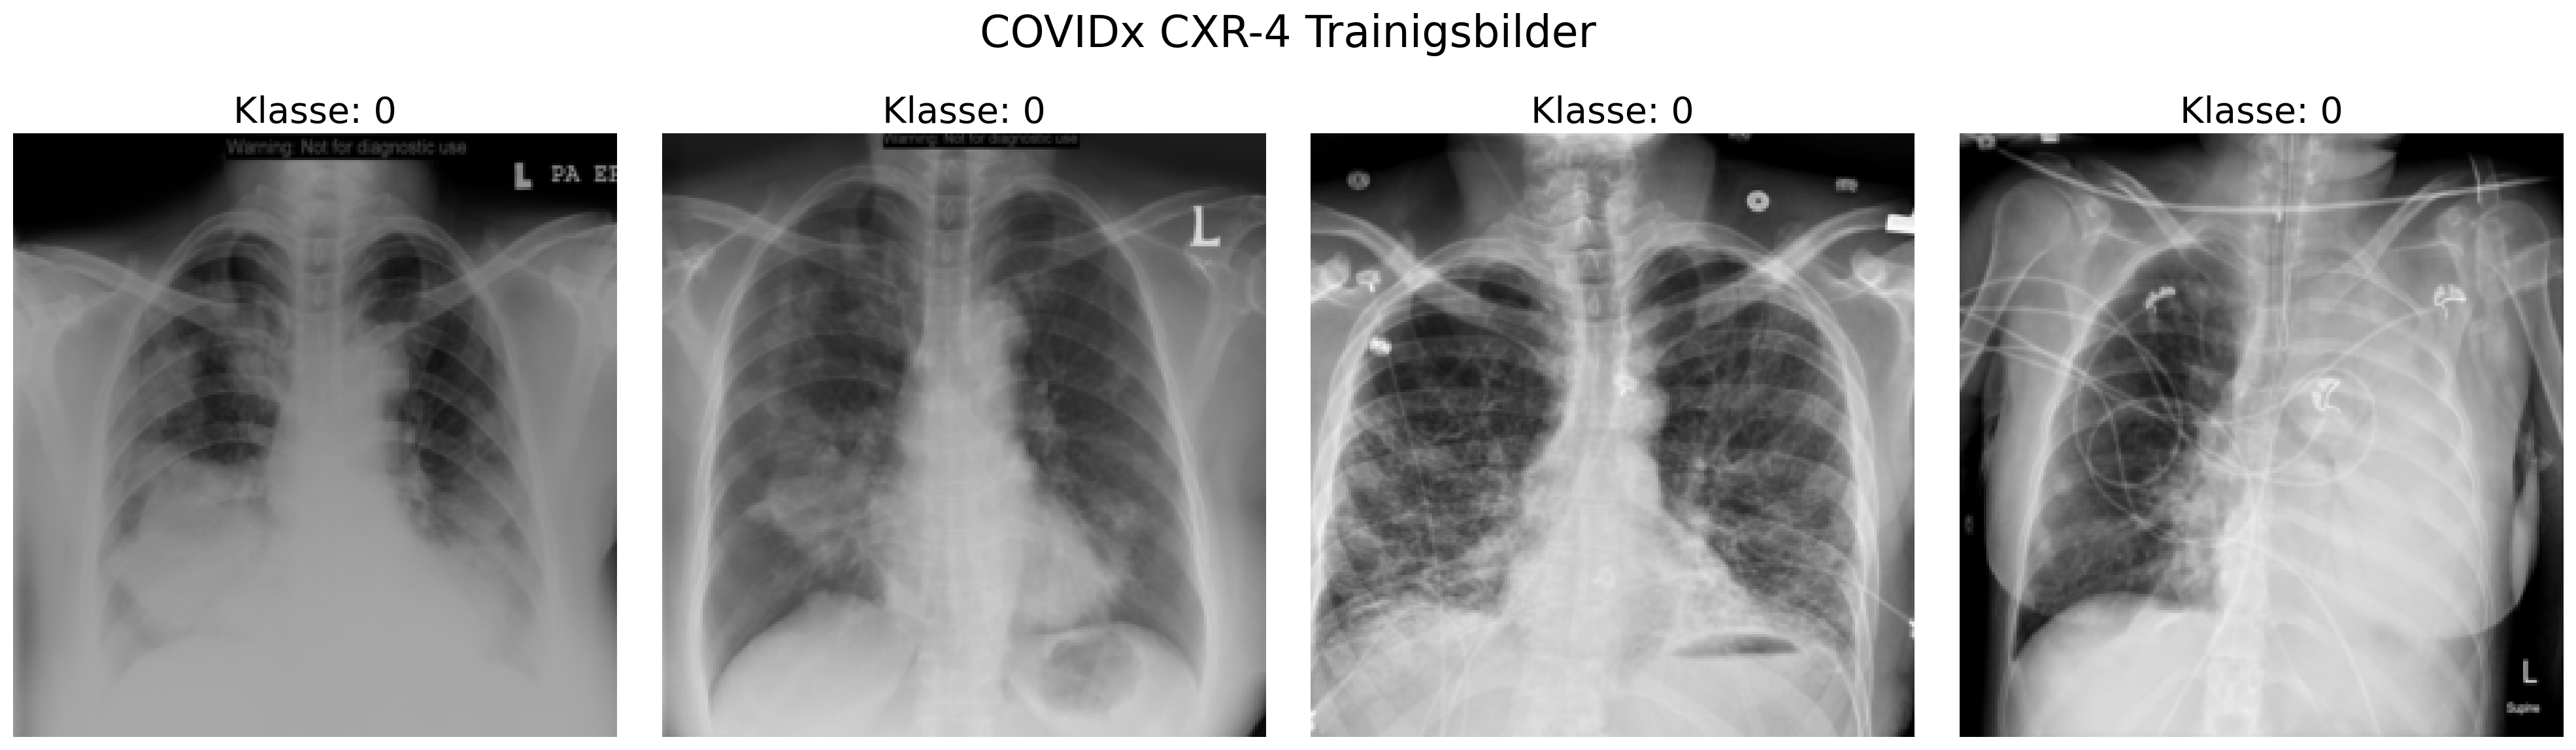
\includegraphics[width=\linewidth]{01-images/03-data/covid19-klasse0.png}
    \caption{Beispiele von negativen Covid Patienten vom COVIDx CXR-4 Datensatz}
    \label{fig:covid19-beispiele-klasse0-negativ}
\end{figure}

\begin{figure}[H]
    \centering
    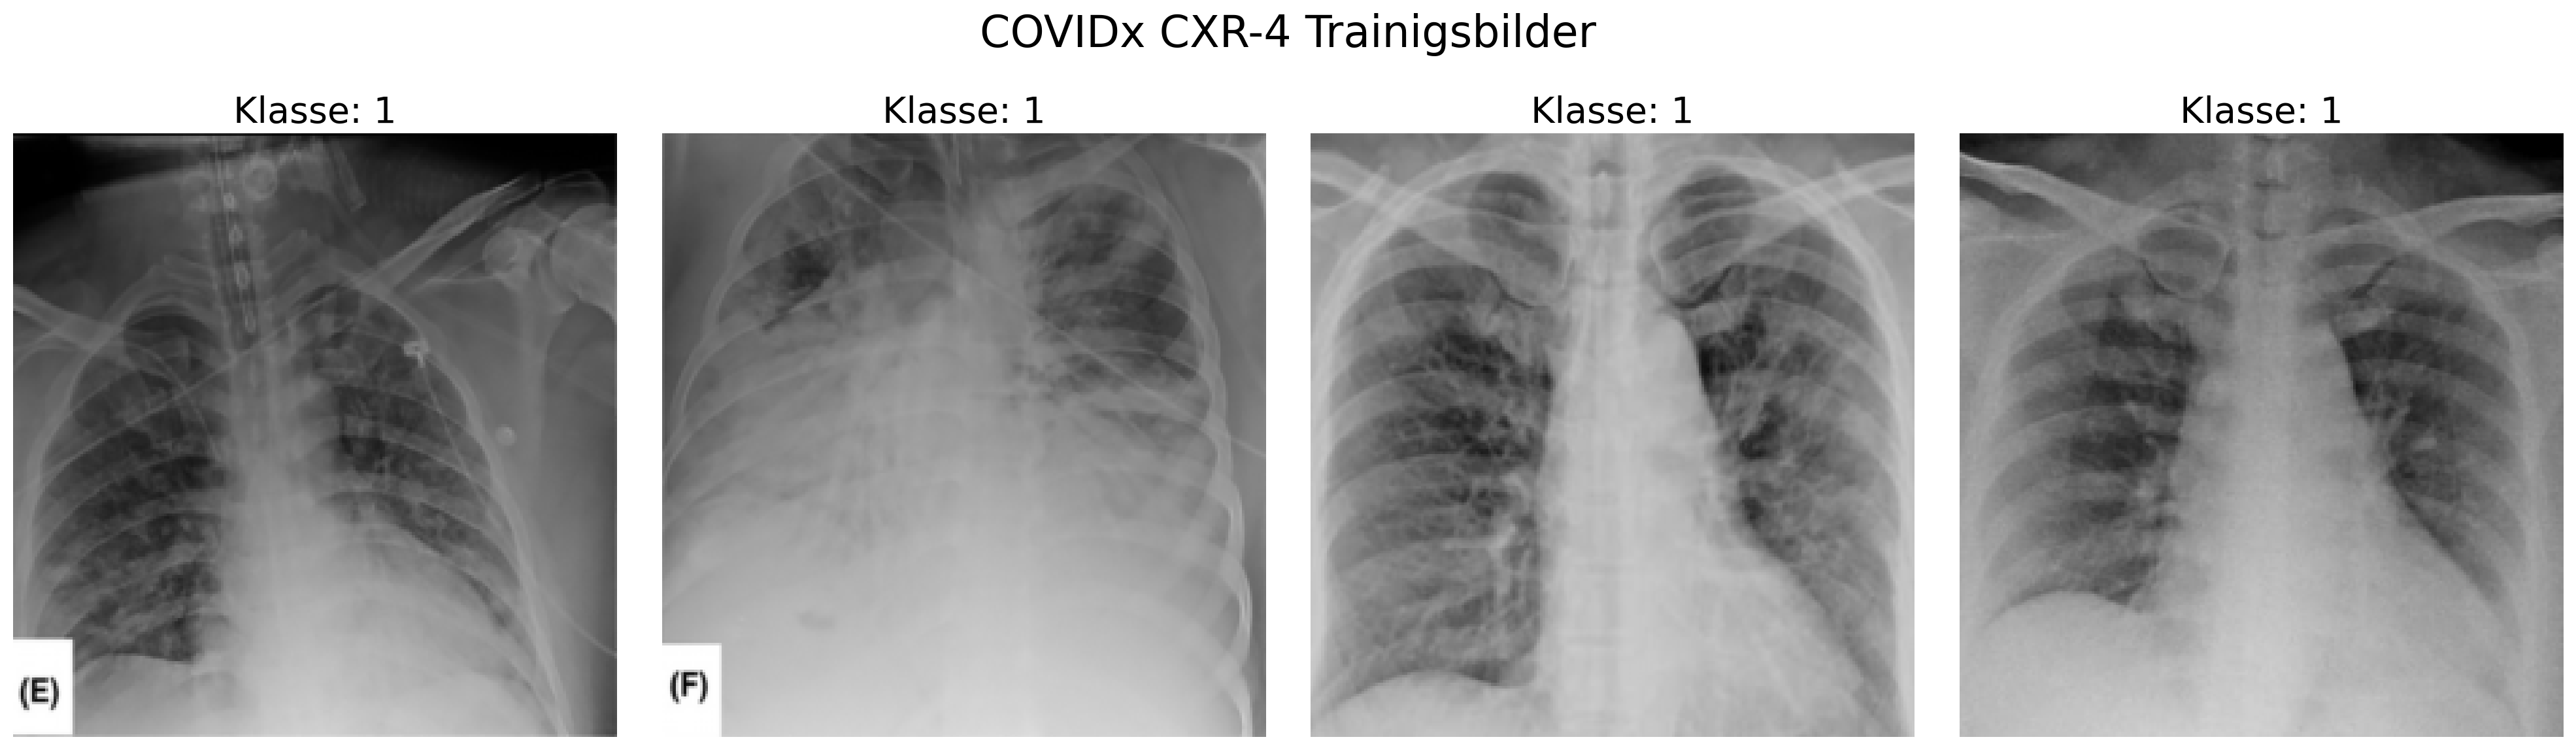
\includegraphics[width=\linewidth]{01-images/03-data/covid19-klasse1.png}
    \caption{Beispiele von positiven Covid Patienten vom COVIDx CXR-4 Datensatz}
    \label{fig:covid19-beispiele-klasse1-positiv}
\end{figure}

\subsubsection{Datenpartitionierung} \label{chap:COVID19-Partition}
Die Datenpartitionierung ist bereits durch die Struktur vorgegeben. Die Klassenverteilung von positiven und negativen Labels für die Validierungs- und Testdatensätze ist nahezu gleich verteilt, mit einem Verhältnis von 50 \% positiven zu 50 \% negativen Fällen.

\begin{table}[h]
    \centering
    \begin{tabular}{@{}cccccc@{}}
        \toprule
        Partition & \multicolumn{2}{c}{Anzahl Bilder} & \multicolumn{2}{c}{Klassenverteilung} & Positiv-Verhältnis\\ 
        \cmidrule(lr){2-3} \cmidrule(lr){4-5} 
                  & Absolut & Relativ & Positiv & Negativ & \\ 
        \midrule
        Train      & 67863 & 0.8001 & 57199 & 10664 & 0.8429 \\
        Validation & 8473  & 0.0999 & 4241  & 4232  & 0.5005 \\
        Test       & 8482  & 0.1000 & 4241  & 4241  & 0.5000 \\ 
        \bottomrule
    \end{tabular}
    \caption{Klassenverteilung von COVIDx CXR-4 Datensatz}
    \label{tab:covid19-klassenverteilung}
\end{table}

\subsubsection{Datenexploration} \label{chap:COVID19-eda}
Die Histogramme in den Abbildungen \ref{fig:covid19-beispiele-klasse0-negativ} und \ref{fig:covid19-beispiele-klasse1-positiv} zeigen die Pixelverteilung der Röntgenbilder von Patienten mit positiven und negativen Testergebnissen. Jedes Histogramm stellt die Intensitätsverteilung der Pixelwerte in den jeweiligen Röntgenaufnahmen dar. Auf der x-Achse jedes Histogramms wird die Grauwertintensität von 0 bis 255 dargestellt, während die y-Achse die Anzahl der Pixel für jede Intensität anzeigt.

\begin{figure}[H]
    \centering
    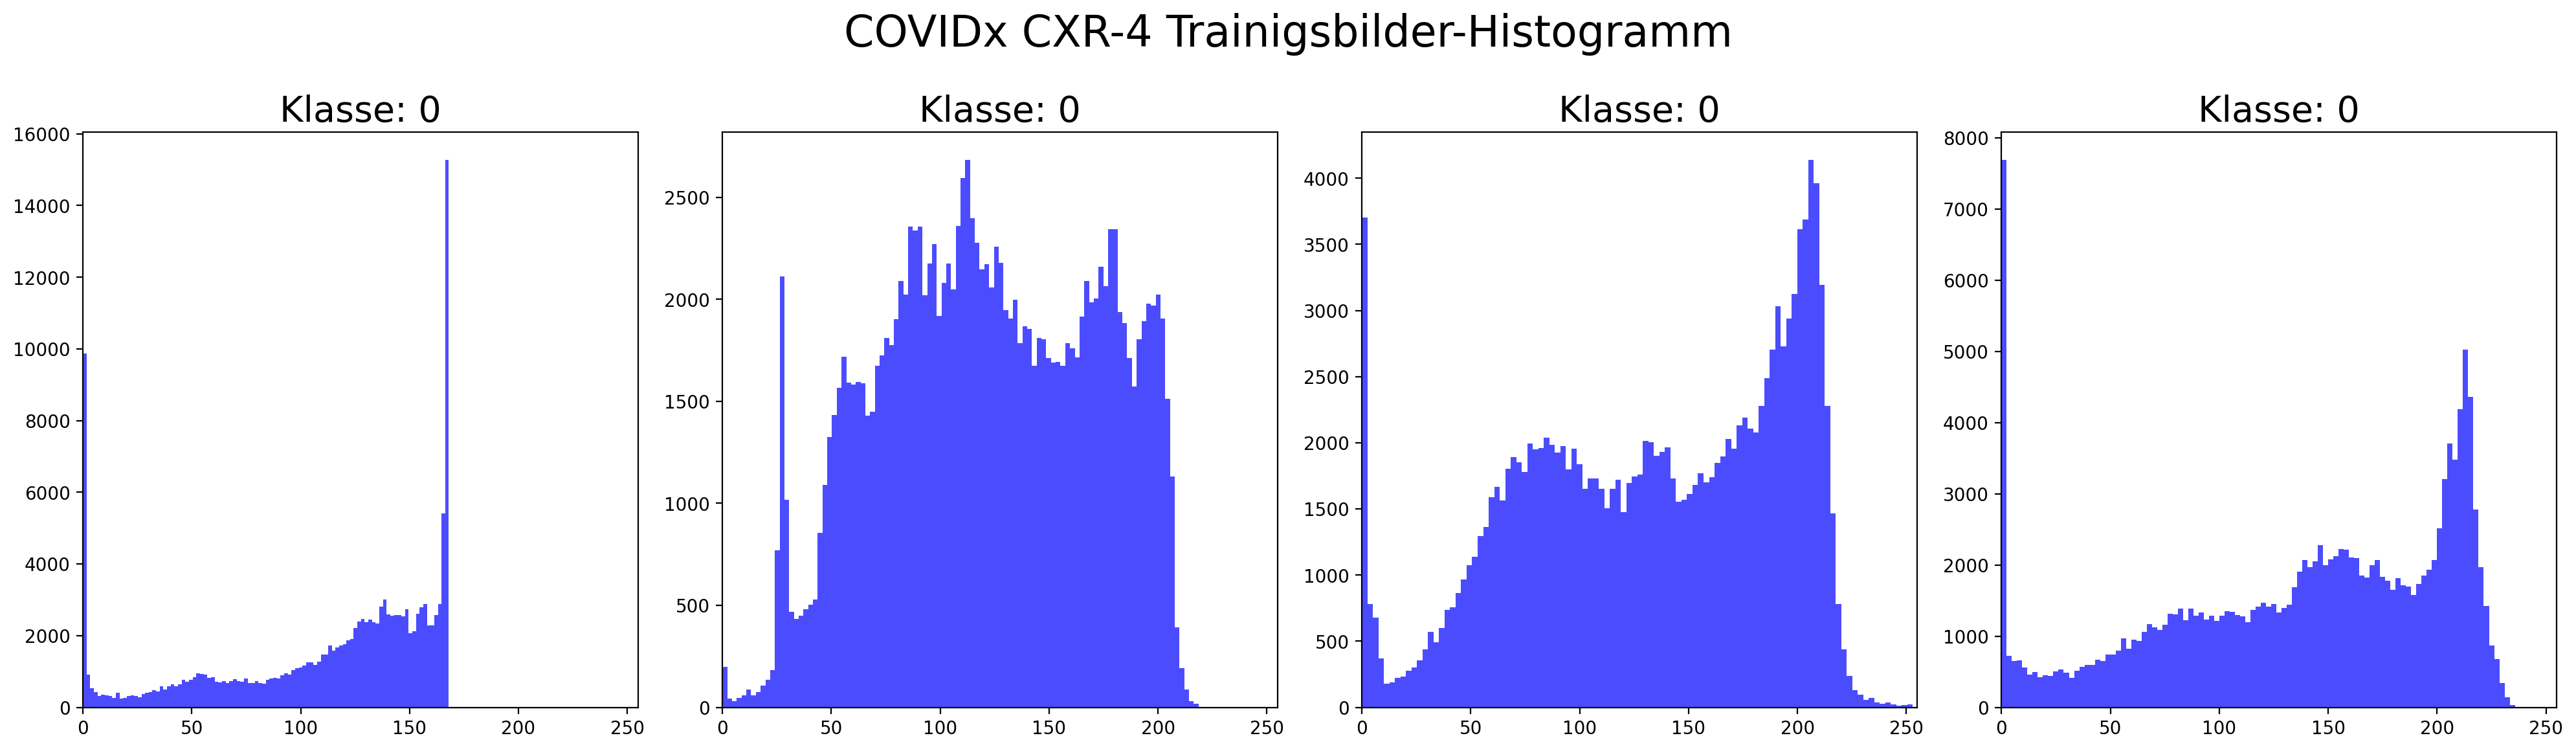
\includegraphics[width=\linewidth]{01-images/03-data/covid19-klasse0-hist.png}
    \caption{Histogramm der Pixelverteilung von Abbildung \ref{fig:covid19-beispiele-klasse0-negativ}}
    \label{fig:covid19-klasse0-hist}
\end{figure}

\begin{figure}[H]
    \centering
    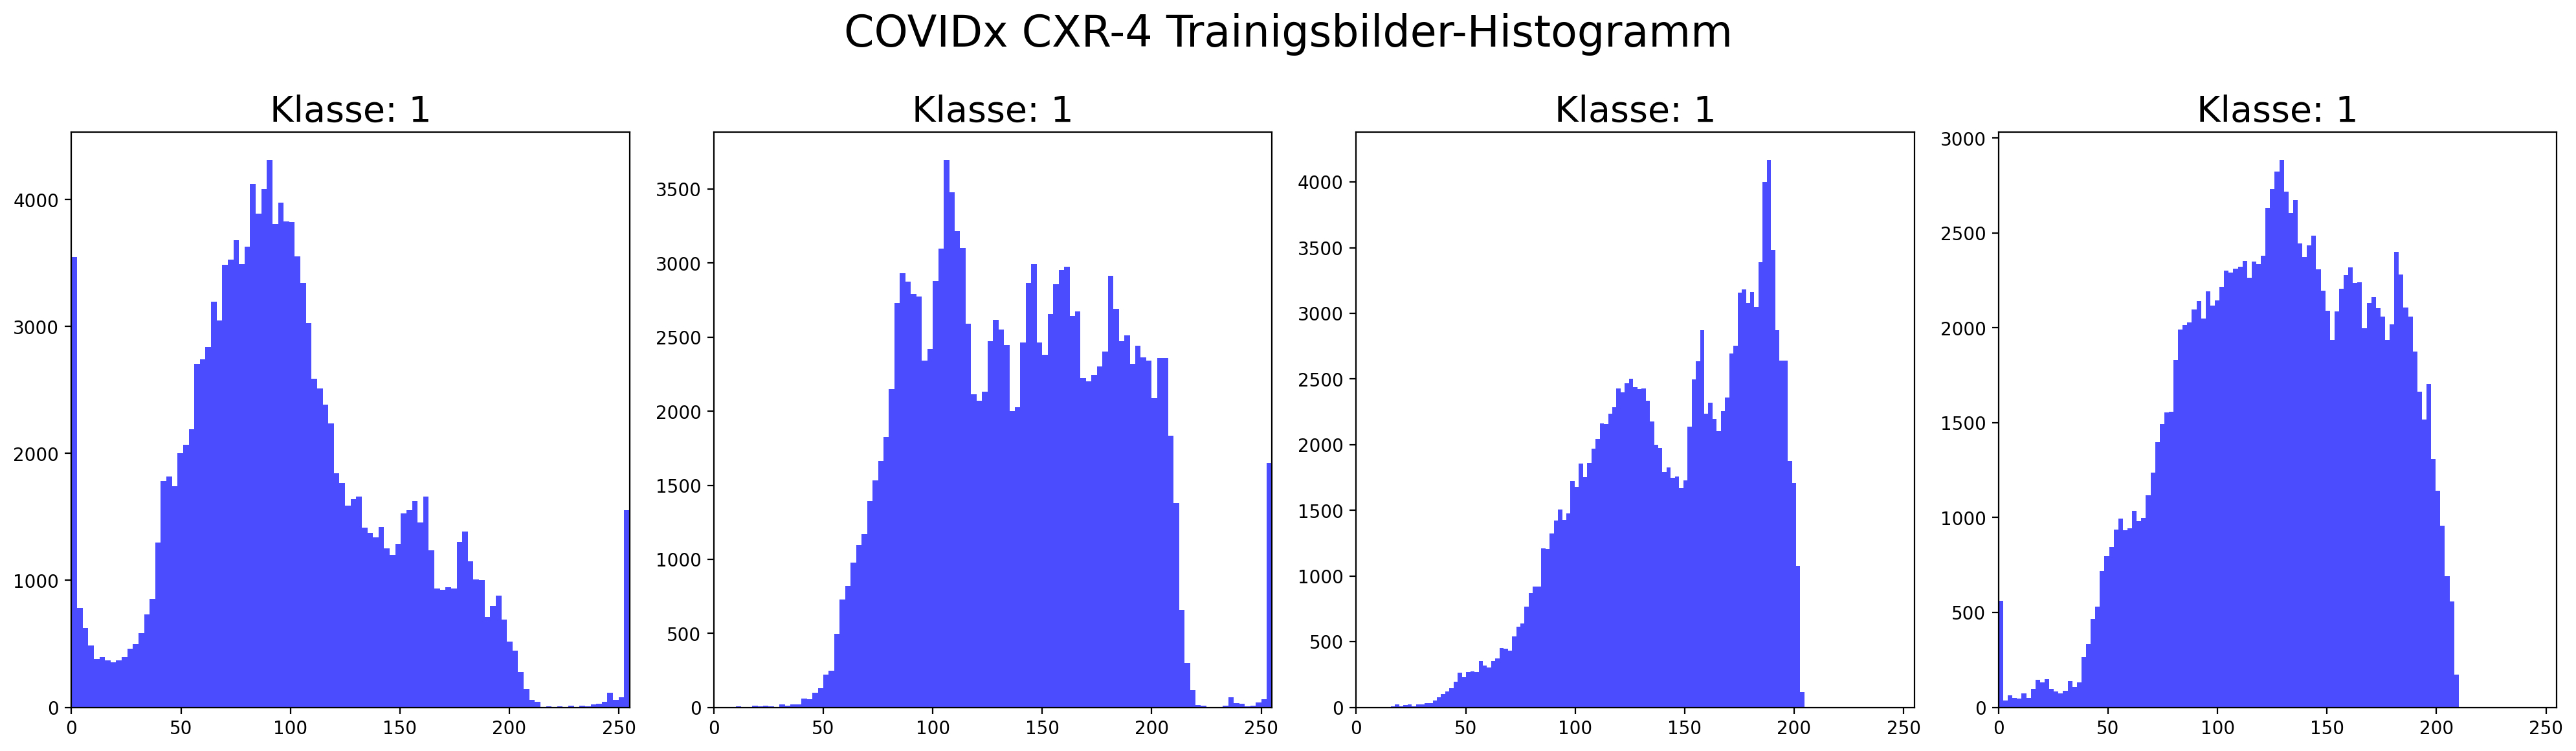
\includegraphics[width=\linewidth]{01-images/03-data/covid19-klasse1-hist.png}
    \caption{Histogramm der Pixelverteilung von Abbildung \ref{fig:covid19-beispiele-klasse1-positiv}}
    \label{fig:covid19-klasse1-hist}
\end{figure}

Die Histogramme der Röntgenbilder zeigen deutliche Unterschiede zwischen den einzelnen Aufnahmen. Niedrige Pixelwerte stehen für Weichgewebe, während hohe Pixelwerte harte Knochengewebe repräsentieren.

\subsubsection{Datenverteilung} \label{chap:COVID19-datenverteilung}
Im Verlauf der Arbeit zeigte sich, dass die Performance Metriken der Testdaten von Covid nicht den erwarteten Werten entsprachen. Daher wurde eine umfassende explorative Analyse der Trainings-, Validierungs- und Testdaten durchgeführt, um potenzielle Ursachen für diese Diskrepanzen zu identifizieren. In den Kapiteln  \ref{chap:COVID19-pixelverteilung}, \ref{chap:COVID-19-pixelmittelwert} und \ref{chap:COVID19-differenzbilder} werden die Ergebnisse dieser Untersuchungen präsentiert.

\paragraph{Pixelverteilung} \label{chap:COVID19-pixelverteilung}
Um die Verteilung der Pixelwerte zu analysieren, werden die Bilder zu eindimensionalen Vektoren abgeflacht. Diese Vektoren repräsentieren alle Bilder der jeweiligen Datenpartition. Die resultierenden Daten werden mithilfe von Histogrammen visualisiert, wie in Abbildung \ref{fig:covid-datapartition-pixelverteilung-histo} dargestellt.

\begin{figure}[H]
    \centering
    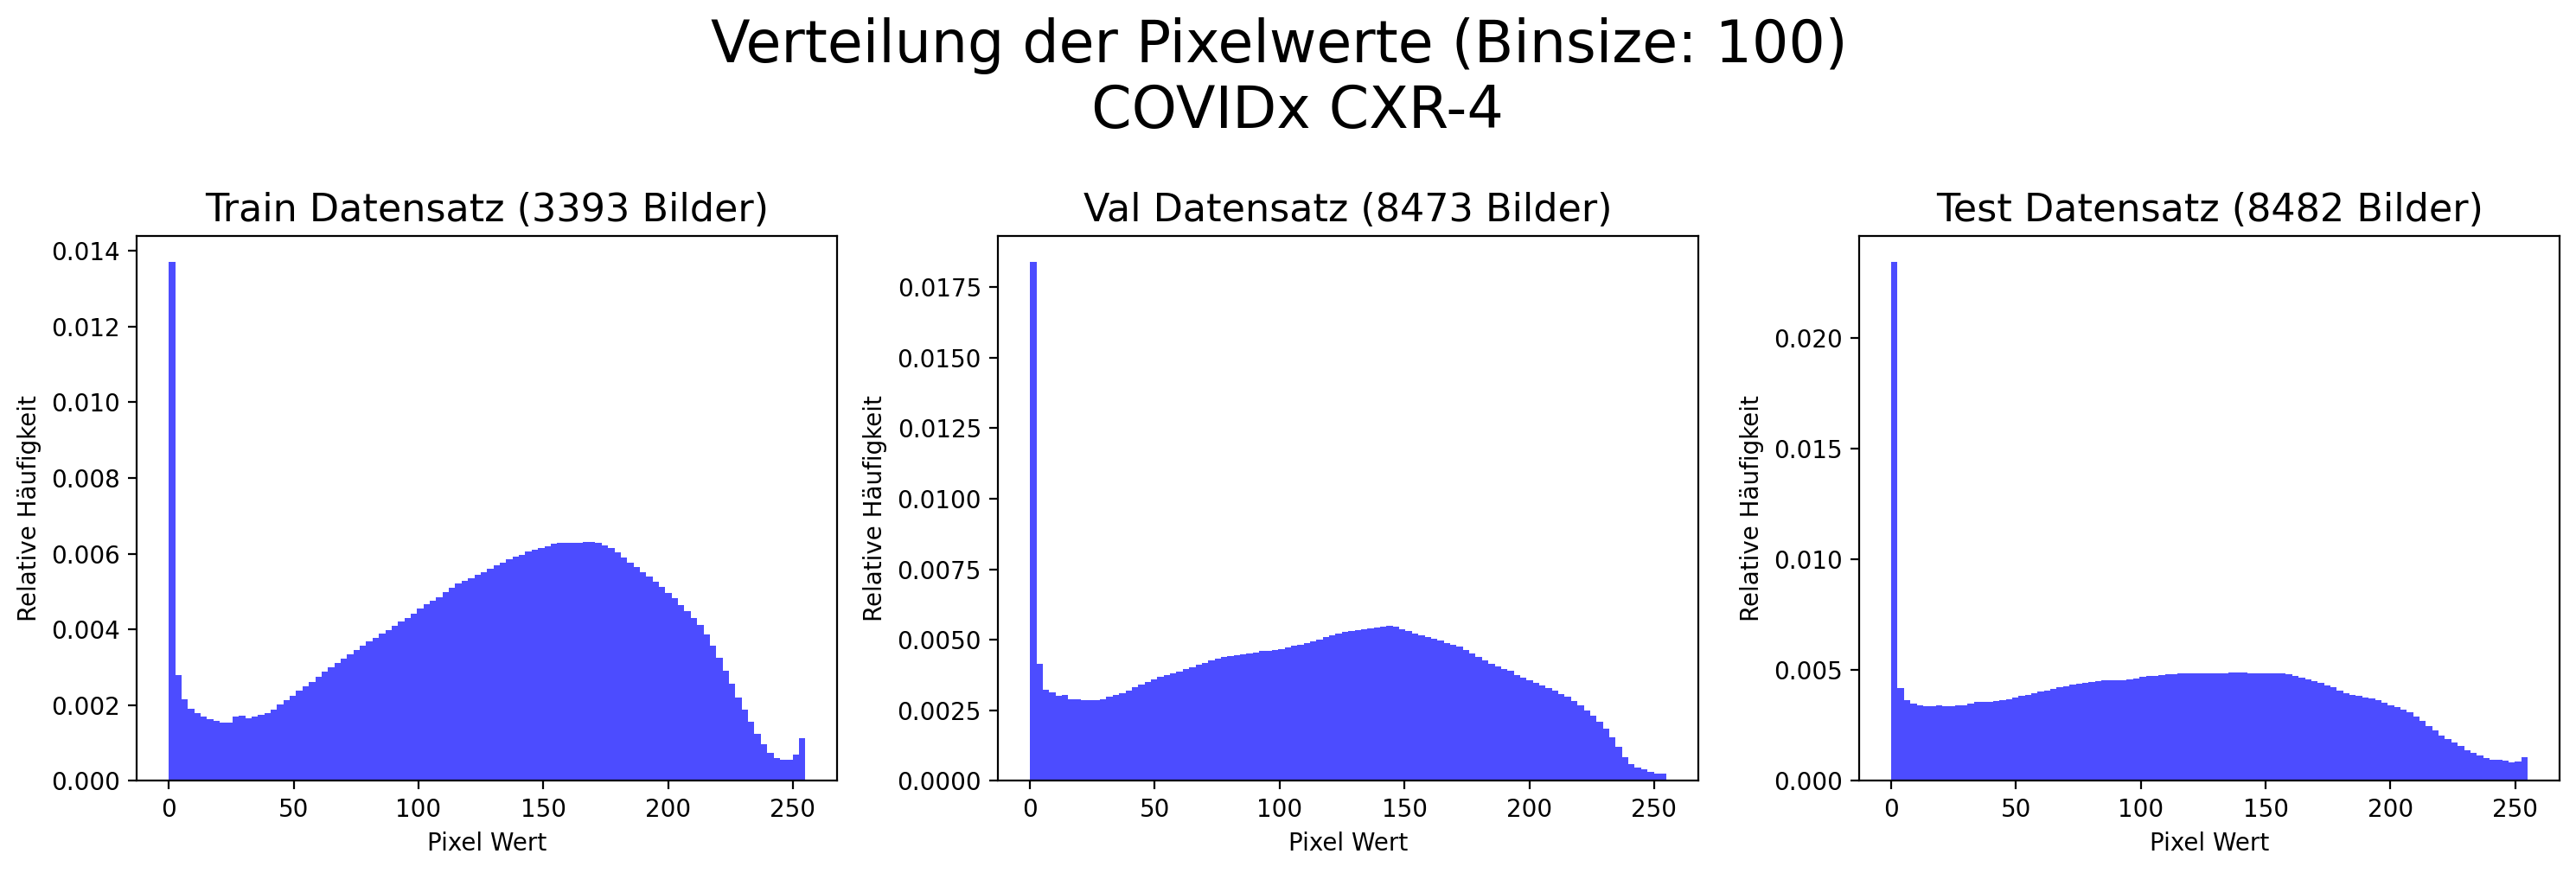
\includegraphics[width=\linewidth]{01-images/03-data/covid-Pixelverteilung-Partitionen.png}
    \caption{Histogramme der Pixelverteilung von Covid in jeder Datenpartition}
    \label{fig:covid-datapartition-pixelverteilung-histo}
\end{figure}

Die Histogramme zeigen, dass Pixelwerte nahe null, die schwarzen Pixeln entsprechen, häufig auftreten, was bei Röntgenaufnahmen üblich ist. Besonders auffällig ist der Gipfel bei einem Pixelwert von etwa 180. Dieser Gipfel ist auch im Validierungsdatensatz vorhanden, jedoch weniger ausgeprägt. Im Testdatensatz ist dieser Gipfel nahezu nicht vorhanden, stattdessen zeigt sich am Ende der Verteilung ein leichter Anstieg, der auf weisse Pixelwerte hinweist. Die Pixelwertverteilungen in den Trainings- und Validierungsdaten zeigen ein ähnliches Muster, jedoch mit unterschiedlichen Intensitäten, was auf Variationen in der Bildaufnahme zwischen den Partitionen hinweisen könnte. Der deutliche Unterschied im Testdatensatz, insbesondere das Fehlen des typischen Gipfels, könnte auf unterschiedliche Charakteristika der Bilder oder eine andere Verteilung in dieser Partition hindeuten. Es ist möglich, dass die Testpartitionen einer anderen Verteilung folgen, was auf verschiedene Faktoren wie Belichtungszeiten, Sensoreinstellungen oder die Art der Datensammlung durch unterschiedliche Maschinen zurückzuführen sein könnte.

\paragraph{Pixelmittelwert} \label{chap:COVID19-pixelmittelwert}
Die Pixelmittelwerte berechnen den durchschnittlichen Pixelwert innerhalb jeder Datenpartition in einer festgelegten Dimension von 224 x 224 Pixeln. Diese spezifische Dimension wurde aufgrund der Anforderungen des Preprocessing Schrittes in der Analyse gewählt. Das Ziel dieser Visualisierung besteht darin, die Unterschiede zwischen den Partitionen auf eine visuell zugängliche Weise darzustellen und dadurch potenzielle Auffälligkeiten oder Muster zu identifizieren.

\begin{figure}[H]
    \centering
    \begin{subfigure}[b]{0.49\linewidth}
        \centering
        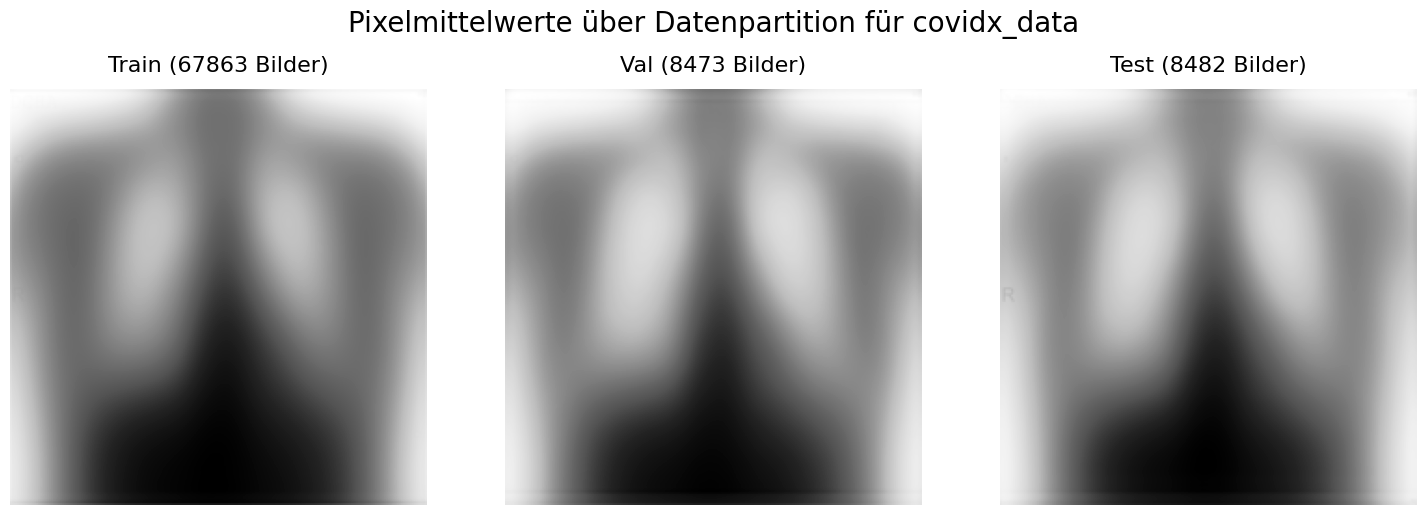
\includegraphics[width=\linewidth]{01-images/03-data/covid-pixelmittelwerte.png}
        \caption{Visuelle Darstellung der Pixelmittelwerte von aller COVID-19-Bildern pro Datenpartition}
        \label{fig:covid-pixelmittelwert-full}
    \end{subfigure}
    \hfill
    \begin{subfigure}[b]{0.49\linewidth}
        \centering
        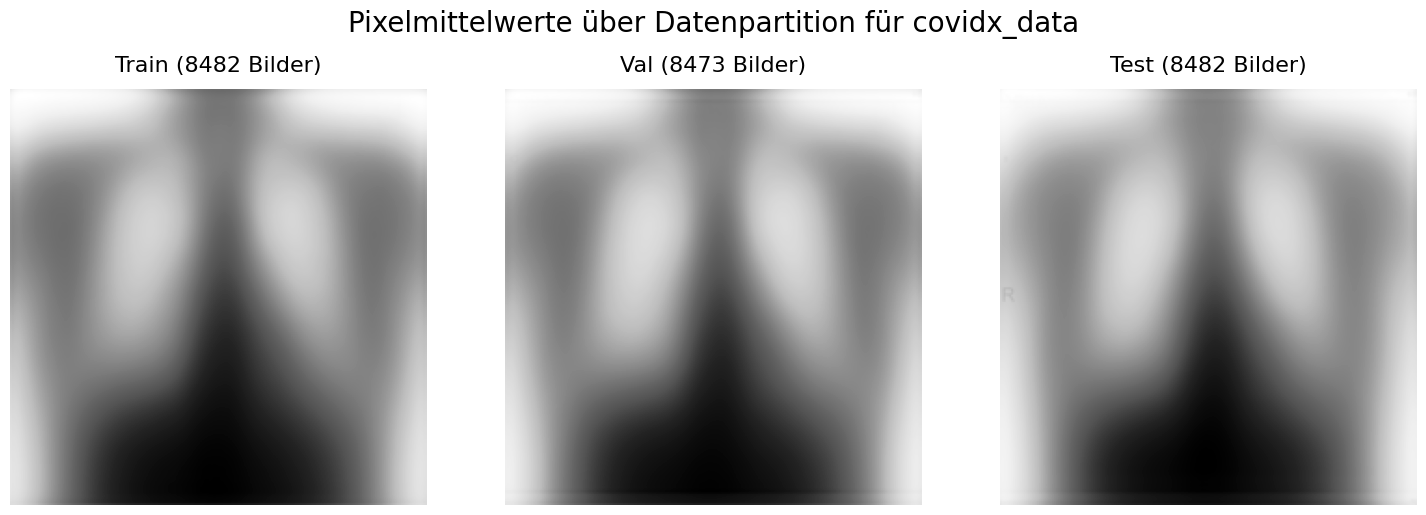
\includegraphics[width=\linewidth]{01-images/03-data/covidx-pixelmittelwert-subsample-train.png}
        \caption{Visuelle Darstellung der Pixelmittelwerte einer Teilmenge von COVID-19-Bildern Datenpartition}
        \label{fig:covid-pixelmittelwert-subsample}
    \end{subfigure}
    \caption{Vergleich der Pixelmittelwerte von COVID-19-Bildern}
    \label{fig:covid-pixelmittelwert-comparison}
\end{figure}

Die Analyse der Pixelmittelwerte über die verschiedenen Datenpartitionen des Covid-Datensatzes zeigt minimale Unterschiede zwischen Trainings-, Validierungs- und Testpartitionen. In allen Partitionen sind beide Lungenflügel sowie das umliegende Bauchgewebe deutlich erkennbar. Die Dunkelheit in der Mitte der Bilder könnte auf die Dichte des Gewebes in diesen Bereichen hindeuten, während hellere Bereiche weniger dichte Gewebe repräsentieren. Die Trainingspartition enthält wesentlich mehr Bilder als die Validierungs- und Testpartitionen. Daher wurde Abbildung \ref{fig:covid-pixelmittelwert-subsample} erstellt, die eine Teilmenge der Trainingsbilder zeigt. Visuell ist kein Unterschied zur gesamten Trainingspartition erkennbar.


\paragraph{Differenzbilder} \label{chap:COVID19-differenzbilder}
Eine weiterführende Analyse der Pixelmittelwerte erfolgt durch die Subtraktion der Werte zwischen den Partitionen. Abbildung \ref{fig:differenz-datapartition-covid} zeigt diese Differenzen als Heatmap. Hierbei werden die Pixelmittelwerte aus Abbildung \ref{fig:covid-pixelmittelwert-full} aller Covid Bilder pro Datenpartition die Differenzen dargestellt.

\begin{figure}[H]
    \centering
    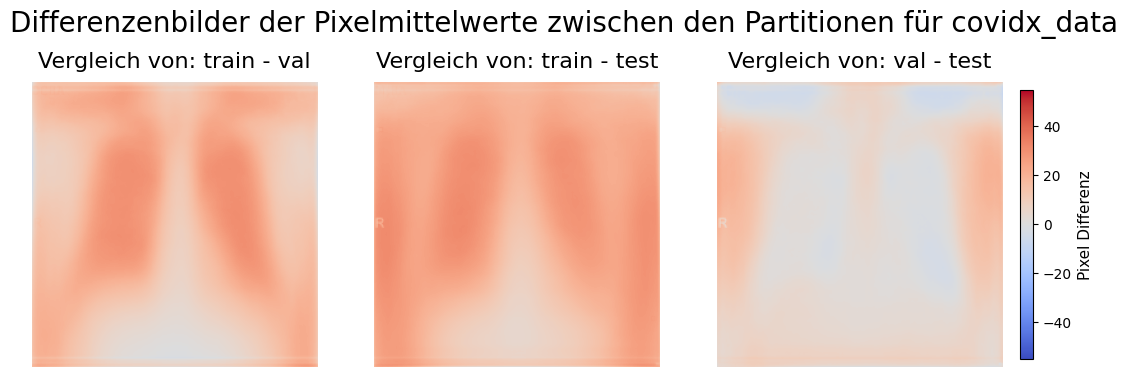
\includegraphics[width=\linewidth]{01-images/03-data/covidx-differenzenbilder.png}
    \caption{Differenzbilder von Covid in jeder Datenpartition}
    \label{fig:differenz-datapartition-covid}
\end{figure}

Der linke Abschnitt veranschaulicht die Differenzen der durchschnittlichen Pixelwerte zwischen Trainings- und Validierungsdaten. Die Berechnung erfolgt durch Subtraktion der Validierungsdaten von den Trainingsdaten. Eine rote Färbung signalisiert höhere durchschnittliche Pixelwerte im Trainingsdatensatz im Vergleich zum Validierungsdatensatz, während eine blaue Färbung niedrigere Werte im Trainingsdatensatz anzeigt.

Im mittleren Abschnitt werden die Differenzen der durchschnittlichen Pixelwerte zwischen Trainings- und Testdaten dargestellt. Die Berechnung erfolgt durch Subtraktion der Testdaten von den Trainingsdaten. Wie im linken Abschnitt kennzeichnen rote Bereiche höhere Pixelwerte im Trainingsdatensatz im Vergleich zum Testdatensatz.

Der rechte Abschnitt zeigt die Differenzen der durchschnittlichen Pixelwerte zwischen Validierungs- und Testdaten. Die Berechnung erfolgt durch Subtraktion der Testdaten von den Validierungsdaten. Ein überwiegend blaues Muster deutet darauf hin, dass die Pixelwerte im Validierungsdatensatz im Durchschnitt niedriger sind als im Testdatensatz.

Diese visuellen Darstellungen der Unterschiede weisen auf potenzielle Verzerrungen und Ungleichgewichte zwischen den Partitionen im Covid Datensatz hin, die die Modellleistung beeinflussen können.

\newpage